\documentclass{article}

\usepackage{graphicx}
\usepackage[a4paper, margin=3cm]{geometry}
\usepackage[hidelinks]{hyperref}

\DeclareMathSymbol{"}{\mathalpha}{letters}{`"}

\title{K0: An investigation into using private tokens\\ on smart contract platforms\\ Version 0.1}
\author{Applied Blockchain}
\date{4 July 2019}

\newcommand{\conc}{\mathbin{\|}}
\newcommand{\code}[1]{\texttt{#1}}

\usepackage[maxbibnames=99,dateabbrev=false,urldate=edtf,seconds=true,backref=true,backend=biber]{biblatex}
\addbibresource{k0.bib}

\begin{document}
\maketitle

\begin{abstract}
Smart contract blockchain platforms enable new kinds of decentralised applications used by mutually distrusting parties. However on most such platforms all transactional data is public, which renders them unusable for use cases requiring privacy. ``Privacy coin'' cryptocurrencies like Zerocash solve this problem for the money transfer use case by enabling private payments on a decentralised (special-purpose) blockchain. We describe an adaptation of this scheme for (general-purpose) smart contract blockchain platforms and propose a slight modification to the protocol to allow the use of private payments as triggers for actions in secondary smart contracts independent of the payment system itself.
\end{abstract}

\section{Introduction}
Blockchains provide a still relatively new paradigm of decentralised applications. Smart-contract platforms in particular allow the creation of a multitude of different types of applications between mutually distrusting parties, e.g. trading platforms or tracking systems for supply chains. However, the fact that in most implementations all the business transactions on a blockchain network are visible to all the members of the network has precluded many potential groups of users from adopting the technology, especially companies who wish to hide their commercial activities from their competitors. Research has shown that the public-key/address pseudonymity provided by most blockchain platforms does not provide much privacy at all because the transaction graph can be analysed. For the original blockchain use case of value transfer, recently this privacy problem has been attempted to be solved by so-called ``privacy coins''. It seems promising to try to bring privacy coin technology to the world of smart contract platforms and explore ways of augmenting smart contracts functionality with private payments. The goal is to enable arbitrary trustless \textit{and} private blockchain applications to be built. This document describes the first iteration of one particular approach of doing that. We adapt the Zerocash scheme so that it can be used on a smart contract platform (with an Ethereum smart contract or a Hyperledger Fabric chaincode at its centre) and describe a way by which private payments in that scheme can be used to trigger actions in separate smart contracts. Please note that this is a rough high-level summary of an early-stage work-in-progress project. It should not be seen as a complete or even fully accurate representation of the codebase, nor as an academic paper in the field of cryptography. We tried to stay as close as possible to Zerocash and its implementation in Zcash, which has been in production for years and for which security proofs exist. However we do not make any claims about the security of the scheme described here at this point. Especially, it has not been security-audited.

\pagebreak

\section{Related work}
This work is based on Zerocash \cite{zerocash} and its implementation in Zcash \cite{zcash}. Miximus \cite{miximus}, ZETH \cite{zeth} and Nightfall \cite{nightfall} are recently released schemes implementing Zerocash or parts of it on Ethereum as well. Zether \cite{zether} follows a different approach to providing confidential payments on smart contract platforms, as does AZTEC \cite{aztec}, which is specifically aimed at being usable and economic on the public Ethereum network. Cloak \cite{cloak} is a protocol for private asset transfers and exchanges, while ZkVM \cite{zkvm} and ZEXE \cite{zexe} are designs for more arbitrary private smart contracts.

\section{High-level overview of Zerocash}

The basis of our design is the decentralized anonymous payment (DAP) scheme described in the Zerocash paper \cite{zerocash} and its implementation in the first version (``Sprout'') of Zcash \cite{zcash}. We quickly summarise the scheme here and glance over some details for the sake of simplicity; for a more detailed description the reader is advised to consult the introductory section in \cite{zerocash}. The main state of the system is a list of note commitments (stored as a Merkle tree) and a list of ``used serial numbers''. The leaves of the Merkle tree represent notes or coins resembling UTXOs in Bitcoin, however while at least the values of the UTXOs are publicly visible in Bitcoin, here notes are binding and hiding commitments (ie. they are indistinguishable from random to observers unable to open the commitments) to the amount value of the note $v$, the owner's public key $a_{pk}$ and a random value $\rho$ (rho). Speaking abstractly, transactions take some of these notes as inputs and produce new output notes. The sum of the values of the inputs must equal the sum of the values of the outputs. Moreover, once a note is used as an input in a transaction, it is ``spent'' and cannot be used any more. To enable this in a private fashion, transactions do not reveal which input notes are spent. Transactions contain the ``serial numbers'' of the input notes (the serial numbers are the result of applying a pseudo-random function to $\rho$ and the private key corresponding to the public key $a_{pk}$), the output note commitments, and a zero-knowledge proof. The proof attests that
\begin{itemize}
\item the creator of the transaction holds the private key corresponding to the input note public keys
\item the owner knows the $\rho$ value and the blinding factor $r$ of each of the input notes
\item the revealed serial numbers correspond to the input notes
\item the input notes are included in the Merkle tree
\item the sum of the input values is equal to the sum of the output values
\item the output note commitments are well-formed, ie. each of them is a commitment to an amount, a newly created $\rho$ and a public key
\end{itemize}

A transaction is valid if this proof can be verified and the serial numbers are not yet in the list of used serial numbers (which prevents double-spending). The result of a valid transaction is that the output note commitments are added to the note commitment Merkle tree and the serial numbers are added to the list of used serial numbers.

In order for the recipient of a payment to be able to spend the funds of an output note later on (by using it as an input in another transaction), they need to know (in addition to their private key) the amount $v$, the value $\rho$ and the commitment blinding factor $r$. Therefore these are transmitted in encrypted form as part of the transaction.

Our contribution is an implementation of this scheme for smart contract platforms, which works with Ethereum and Hyperledger Fabric with small adjustments. Moreover, we add support for use cases where private payments on the system can be used as events to trigger actions in other smart contracts.

\section{Description of our adaptation of Zerocash for smart contract platforms and our protocol modification}

\subsection{Components} \label{components}
We target smart contract platforms such as Ethereum \cite{ethereum} and Hyperledger Fabric \cite{fabric}. In order to be able to discuss these more generally, we define two major abstract components:
\begin{itemize}
    \item A \textit{platform}, which can be seen as a ``decentralised application server'', but for the purposes of this description acts like a singleton entity. It holds the state (memory) for the scheme described here (in particular, the note commitment Merkle tree and the list of used serial numbers) and runs code (``smart contracts'') triggered by function calls sent by the nodes. One important responsibility of the platform is to verify zero-knowledge proofs. 
    \item \textit{Nodes} which can send messages (function calls) to the platform and receive messages (events) from the platform. Typically every user of the system will have their own node. Nodes also need memory, to hold some state about the system and more importantly the user's secrets (private key and for each note $\rho$, $v$ and $r$). In preparation to calling functions, nodes may generate zero-knowledge proofs.
\end{itemize}

A function call from a node triggers code on the platform to be executed, which may result in state changes and events broadcast to all the nodes. Every function call / state change / event emission cycle constitutes a \textit{transaction}. Transactions are executed atomically and sequentially, usually the consensus mechanism of the blockchain will determine the order of transactions.

One important aspect of the smart contract platform is that it allows different types of ``programs'' (smart contracts) to be available in the system, and that smart contract code that gets executed during a transaction  may itself send function call messages to other smart contracts, which will be processed in the same transaction.

The scheme discussed here assumes transactions can be sent anonymously and without cost. In private/consortium Ethereum setups this is usually not an issue, however in public Ethereum every transaction costs a certain amount of Ether, and this Ether has to be acquired from somewhere beforehand, which represents a challenge to anonymity. However there are ideas of overcoming these limitations, for example by the use of transaction relayers. In Hyperledger Fabric, relayers could be used as well, another option would be the use of the ``Identity Mixer'' technology.

\subsection{Operations} \label{operations}
The following describes the operations offered by the system. Most of the processes are almost identical to those of Zerocash and Zcash, therefore the reader is referred to \cite{zerocash} and \cite{zcash} for a more detailed description.

\subsubsection{Platform initialisation}
The platform gets initialised with an empty note commitment Merkle tree and an empty list of used serial numbers.
\subsubsection{Key generation} \label{keygeneration}

To participate in the system, a user needs to sample a random note private key (or, in Zcash parlance, spending key) $a_{sk}$ from which the following keys are derived:
\begin{itemize}
    \item $a_{pk} := H(a_{sk} \conc 0^{256})$ (note public key or paying key)
    \item $sk_{enc} := SkEncGen(a_{sk})$ (encryption private key or receiving key)
    \item $pk_{enc} := PkEncGen(sk_{enc})$ (encryption public key or transmission key)
\end{itemize}

$SkEncGen$ is the private encryption key derivation function and $PkEncGen$ is the public encryption key derivation function (see section \ref{encryption}).
$a_{sk}$ and $sk_{enc}$ must always be kept private (known only to the user). $a_{pk}$ and $pk_{enc}$ get concatenated to form a \textit{K0 address}:
$$addr := a_{pk} \conc pk_{enc}$$
\subsubsection{Mint (Deposit)} \label{mint}
As a store of value, the K0 system needs to provide a way to create or ``mint'' tokens. Viewed abstractly, the problem that needs to be solved is that a certain value needs to be added to a particular user's balance. How this is triggered differs in the implementations:
\begin{itemize}
    \item In the Ethereum version the private token is ``backed'' by a regular ERC-20 token. A user is entitled to ``mint'' a certain amount of private coins by ``locking up'' an equivalent amount of the ERC-20 token in the smart contract (similarly she can later withdraw her ERC-20 token value again by ``burning'' an equivalent amount of private token value, see section \ref{burn}). This mechanism essentially allows us to delegate the question of overall money supply and minting to the backing ERC-20 token.
    \item In the Fabric version (since there is no notion of smart contracts having native ``accounts'' which would allow a scheme of ``locking up'' value) one trusted ``minter'' organisation is entitled to mint all the value.
\end{itemize}
In both cases, the minting operation will increase the money supply by a publicly visible amount, and will ensure that this amount is subsequently spendable by a certain user whose identity is only known to the user herself and the ``minter'' (in the Ethereum version one would typically mint money for oneself). In particular, the minter samples a randomness $\rho$ and creates a commitment $k$ to $\rho$ and the recipient's note public key $a_{pk}$ using a hash function\footnote{Currently instantiated with the compression function of SHA256} and a blinding factor $r$\footnote{$[\cdot]_x$ denotes truncating a longer bit string to $x$ bits.}:
\[ k := H(r \conc [H(a_{pk} \conc \rho)]_{128}) \]
He then creates a commitment $cm$ to $k$ and the minted value $v$:
\[ cm := H(k \conc 0^{192} \conc v) \]
The minter then sends $v$, $k$, $cm$ and some encrypted $data$ to the smart contract in a call to the function $mint$:
\[ mint(v, k, cm, data) \]
$data$ contains the values $v$\footnote{$v$ is not strictly needed here because it is included in the public parameters to the function call, but is included for simplicity reasons as the same encryption/decryption code can be used for the transfer function (where $v$ is hidden), see \ref{transfer}.}, $\rho$ and $r$ encrypted with the recipient's encryption public key $pk_{enc}$\footnote{There is no check in the system that ensures that data is actually the encryption of $v$, $\rho$ and $r$. This means it is possible that some undecipherable data can be sent in this field. This will result in the recipient not being able to spend the note or even being notified of the payment. However when the intention is to ``send someone money'', there is no reason to do that. Should sender and recipient not want to trust the security of the encryption scheme or its implementation, they can choose to ignore this field and transmit the values through some other mechanism out-of-band.}.
The smart contract checks that $cm$ equals $H(k \conc v)$. If this check succeeds, it adds $cm$ to a list of note commitments, stored as a Merkle tree, and emits a \textit{Mint} event containing $cm$ and $data$ as payload. Upon receiving this event, the recipient of the note will be able to decrypt $data$ using their secret key $sk_{enc}$ and store the values $v$, $\rho$ and $r$ in a database that relates them to the note commitment $cm$ and its position in the Merkle tree.


\subsubsection{Transfer} \label{transfer}
A transfer operation ``consumes'' or ``spends'' two ``input'' notes and creates two new ``output'' notes\footnote{The restriction on two input notes and two output notes is due to the requirement of having a fixed circuit for the zero-knowledge proof.}. The output notes will be added to the Merkle tree. It will not be revealed which of the available notes are used as the input notes, however for each of them their ``serial number'' will be revealed. The system keeps track of the serial numbers, which prevents double spending. Moreover the transfer operation will ensure that the user sending the transaction is actually entitled to spend the input notes, and that the sum of the values of the input notes matches the sum of the values of the output notes (ie. no money is created or lost in the process).
In detail, a transfer operation is created in the following steps: A user (or rather, his wallet software) selects from his database two input notes for which he holds the private values $v_1^{in}$, $\rho_1^{in}$, $r_1^{in}$ and $v_2^{in}$, $\rho_2^{in}$, $r_2^{in}$, respectively. He creates two output notes (typically one representing the intended payment to another user, and one ``change'' output for himself) by setting $v_1^{out}$ and $v_2^{out}$ and sampling  $\rho_1^{out}$, $\rho_2^{out}$, $r_1^{out}$ and $r_2^{out}$.

He creates a proof $\pi$ that attests:
Given Merkle tree root $rt$, values $sn_1^{in}$, $sn_2^{in}$, $cm_1^{out}$, $cm_2^{out}$ and $id_{callee}$, I know input note info
($a_{pk}^{in}$, $v_1^{in}$, $\rho_1^{in}$, $r_1^{in}$, $cm_1^{in}$),
($a_{pk}^{in}$, $v_2^{in}$, $\rho_2^{in}$, $r_2^{in}$, $cm_1^{in}$),
output note info 
($a_{pk,1}^{out}$, $v_1^{out}$, $\rho_1^{out}$, $r_1^{out}$),
($a_{pk,2}^{out}$, $v_1^{out}$, $\rho_1^{out}$, $r_1^{out}$),
Merkle tree paths $path_1$ and $path_2$, note private key $a_{sk}$ and value $id_{callee}^{private}$ s.t.:
\begin{itemize}
    \item The coins are well-formed:
    \begin{itemize}
        \item $cm_1^{in} = H(H(r_1^{in} \conc [H(a_{pk,1}^{in} \conc \rho_1^{in})]_{128}) \conc 0^{192} \conc v_1^{in})$
        \item $cm_2^{in} = H(H(r_2^{in} \conc [H(a_{pk,2}^{in} \conc \rho_2^{in})]_{128}) \conc 0^{192} \conc v_2^{in})$
        \item $cm_1^{out} = H(H(r_1^{out} \conc [H(a_{pk,1}^{out} \conc \rho_1^{out})]_{128}) \conc 0^{192} \conc v_1^{out})$
        \item $cm_2^{out} = H(H(r_2^{out} \conc [H(a_{pk,2}^{out} \conc \rho_2^{out})]_{128}) \conc 0^{192} \conc v_2^{out})$
    \end{itemize}
    \item My private key corresponds to the public key of the input notes: $a_{pk}^{in} = H(a_{sk} \conc 0^{256})$
    \item{The serial numbers are computed correctly\footnote{As pointed out in \cite{zeth}, the fact that only 254 bits of $\rho$ are used here creates an attack vector which allows a sender to create multiple notes with the same serial number. We aim to address this issue in a future version of the protocol.}:
    \begin{itemize}
        \item $sn_1^{in} = H(a_{sk} \conc 0 \conc 1 \conc [\rho_1^{in}]_{254})$
        \item $sn_2^{in} = H(a_{sk} \conc 0 \conc 1 \conc [\rho_2^{in}]_{254})$
    \end{itemize}}
    \item $cm_1^{in}$ and $cm_2^{in}$ are in the Merkle tree (ie. in a Merkle tree with root $rt$, $path_1$ is a path to leaf $cm_1^{in}$ and $path_2$ is a path to leaf $cm_2^{in}$)
    \item The value of $id_{callee}$ is fixed for the proof: $id_{callee}$ = $id_{callee}^{private}$ (these values will be needed for the ``smart payment'' feature described in section \ref{smartpayment} and will be 0 for this use case)
\end{itemize}
The sender then calls the transfer smart contract function with the following call: $$transfer(sn_1^{in}, sn_2^{in}, cm_1^{out}, cm_2^{out}, data_1^{out}, data_2^{out}, rt_{new}, id_{callee}, \pi).$$ $data_1^{out}$ and $data_2^{out}$ are the encrypted values $v$, $\rho$, $r$ of the output values (see section \ref{mint}). $rt_{new}$ is the expected root of the Merkle tree after adding $cm_1^{out}$ and $cm_2^{out}$. In this use case, $id_{callee}$ will be set to 0 and therefore will be ignored by the smart contract. $\pi$ is the proof described above. The smart contract will
\begin{itemize}
    \item check that the serial numbers are not yet in the list of used serial numbers
    \item verify the proof with the current Merkle tree root $rt$ and the $sn$ values from the transaction as public inputs
    \item add the serial numbers to the list of used serial numbers
    \item add the note commitments to the Merkle tree
    \item emit a \textit{Transfer} event with the payload $(sn_1^{in}, sn_2^{in}, cm_1^{out}, cm_2^{out}, data_1^{out}, data_2^{out})$.
\end{itemize}
Recipients will be able to decrypt and add to their database the $v$, $\rho$ and $r$ values encrypted in the respective $data$ field of the \textit{Transfer} event. The senders will be able to identify and mark the input notes as spent by the $sn$ values.
\begin{figure}
\centering
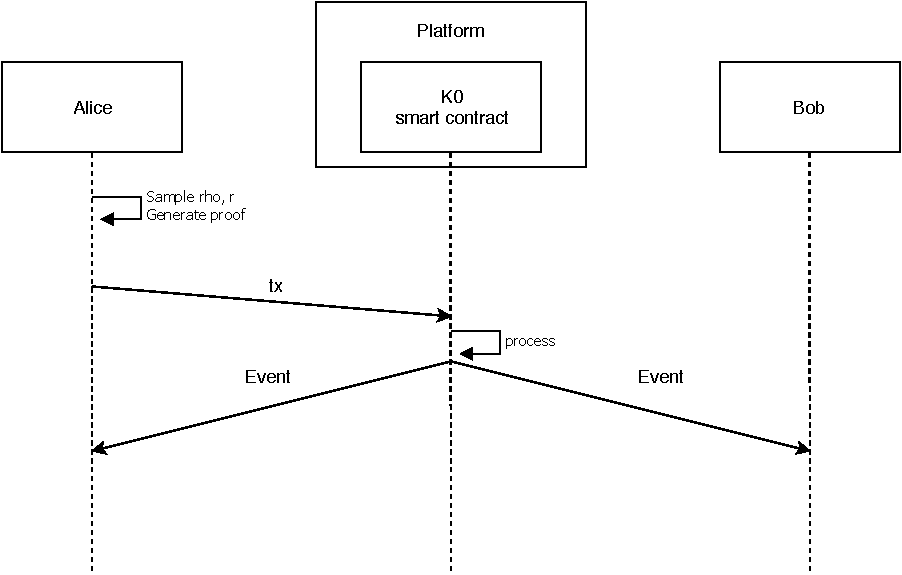
\includegraphics[width=\columnwidth]{payment.pdf}
\caption{A payment flow.}
\end{figure}
\subsubsection{``Smart payment''} \label{smartpayment}
Now let us assume a scenario where the recipient expects a certain payment (for example, a certain amount in exchange for some goods). In this case the party expecting the payment will typically communicate to the sender the value $v$ and their public key $a_{pk}$. Recall that according to the transfer flow described in the previous section, the sender will then sample $\rho$ and $r$, use these values to generate the payment and send them (and the amount $v$) to the recipient (in encrypted form as part of the transfer event). After this has happened, both sender and receiver have knowledge of $v$, $\rho$ and $r$ (but only the receiver will be able to spend the note using their private key). We can modify this process slightly by switching the responsibility of generating $\rho$ and $r$ from the sender to the recipient, ie. the party expecting the payment samples $\rho$ and $r$, and sends $v$, $\rho$, $r$ and $a_{pk}$ to the sender. The sender will then use all these values in the payment. The result in terms of informational insight into the payment for the participating parties is the same, both know $v$, $\rho$ and $r$, but only the recipient can spend the funds later using their private key. However this flow has the interesting property that the party expecting the payment can already precompute for themselves the $cm$ value that will appear in the Merkle tree once the payment is added to the ledger. More importantly, in a smart contract system, they can register that particular $cm$ in another smart contract. Later this smart contract can be convinced (for example through a proof asserting that the $cm$ is included in the Merkle tree whose root $rt$ the smart contract can query) that the payment has happened and, for instance, trigger some action for which the payment was a precondition. Lastly, if the action of informing a smart contract that a certain payment has happened and triggering it to act on it can be in included in the payment transaction itself, the payment and the action that is triggered by it can be modeled as an atomic operation. This is what the $id_{callee}$ parameter in the transfer operation is for: If it is set, the system will call the function $handle(cm)$ on the smart contract specified by $id_{callee}$ (in the Ethereum case, a contract address). The rest of the processing is similar to the normal payment case described in section \ref{transfer}. Note that the transaction is atomic, it will only have an effect if both the transfer and the triggered operation in the secondary contract succeed.

In the test and demo code for our current Ethereum implementation, this functionality is used to achieve a half-private atomic token transfer between the private payment token described here and a non-fungible ERC-721 token. The use case is that a holder of an instance of a certain ERC-721 token wants to offer that token instance (in our example, a ``CarToken'' representing a car, maybe in an on-chain game, or even a real-world ``tokenised'' car, for example in a trading application) for a certain amount of private token through a smart contract facilitating an atomic swap to a selected audience (without revealing anything about the monetary value to anybody else). First she samples $\rho$ and $r$ and generates the commitment $cm$ using these values, the desired price $v$ and her K0 address. She sets up a smart contract that will release the CarToken to the sender of a transaction resulting in $cm$ and shares the values $\rho$, $r$ and $v$ with one or more potential buyers. She also needs to allow this smart contract to transfer the CarToken on her behalf (this functionality is part of the ERC-721 token standard). When the buyer sends the payment, he includes the car trading smart contract address in the $id_{callee}$ field. While processing the transaction, the K0 token smart contract will call the function $handle$ on the car trading contract, which will transfer the CarToken from the seller to the  sender of the transaction, ie. the buyer. Note that this does not hide the identity of the traded CarToken. Also the Ethereum addresses of the old and new owner of the CarToken are public, however (assuming transactions can be sent anonymously, see section \ref{components}) the anonymity provided by the pseudonymity of the Ethereum addresses in this case is assumed to be much stronger than usual as there is no real ``transaction graph'' as the payments are hidden (especially if the adresses are \textit{only} used to aqcuire, hold and dispose of the CarToken).
\begin{figure}
\centering
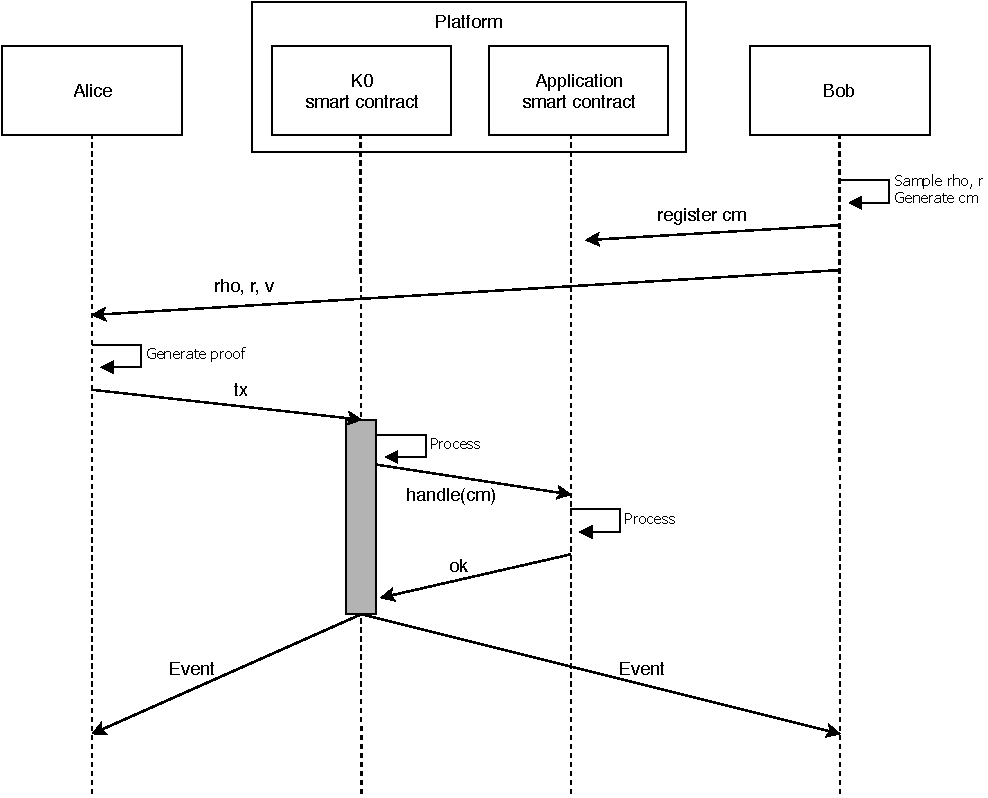
\includegraphics[width=\columnwidth]{smart_payment.pdf}
\caption{A ``smart payment'' flow.}
\end{figure}

\pagebreak

\subsubsection{Burn (Withdraw)} \label{burn}
The system allows users to reduce the overall money supply by ``burning'' notes, ie. spending a note (and revealing its serial number) without creating any new notes. In the Ethereum version backed by an ERC-20 token, this constitutes a withdrawal operation, ie. they will be able to redeem the equivalent amount of ERC-20 token from the pool of deposits.
To burn a note, a user needs to call the smart contract function $burn$: $$burn(v, sn, \pi)$$ $v$ is the value of the note to be burned. $sn$ is the serial number of the note to be burned. $\pi$ is a proof attesting the following: Given values $rt$, $v$, $sn$ and  $id_{sender}$ I know note info $(a_{pk}, \rho, r, cm)$, private key $a_{sk}$ and $id_{sender}^{private}$ s.t.
\begin{itemize}
    \item $cm = H(H(r \conc [H(a_pk \conc \rho)]_{128}) \conc 0^{192} \conc v)$
    \item $a_{pk} = H(a_{sk} \conc 0^{256})$
    \item $sn = H(a_sk \conc 0 \conc 1 \conc [\rho]_{254})$
    \item $cm$ appears in the Merkle tree with root $rt$
    \item $id_{sender} = id_{sender}^{private}$
\end{itemize}
$id_{sender}$ is the sender of the transaction identified by the smart contract and will be added as a public input to the proof verification. It is included in the proof generation to prevent the usage of the proof in another transaction paying out to another user. If the proof verification succeeds, the smart contract adds $sn$ to the list of serial numbers and decreases the overall money supply by $v$. In the Ethereum case it also transfers the ERC-20 value equivalent to $v$ to the account of the sender of the transaction. A \textit{Burn} event is emitted with ${sn}$ as the payload. The sender's node software will be able to identify the input note by the $sn$ and mark it as spent in the database.
\subsection{Additional proofs}
The current implementation deviates a bit from the scheme provided so far. This is due to decisions made to speed up the development process; it meant that we did not need to implement Merkle tree functionality on the smart contract platforms and were able to use the SHA256 compression function in our Merkle tree and the corresponding proofs. The modifications should not constitute a big qualitative difference and will probably be reverted in a later revision: The platform does not store the Merkle tree itself, but only its root $rt$. Nodes have to maintain a copy of the full Merkle tree and update it on each \textit{Mint}/\textit{Transfer}/\textit{Burn} event emitted from the platform.
During the mint operation, the transaction sender provides a proof $\pi_{1}$ that the addition of $cm$ to the Merkle tree $rt$ results in a new Merkle tree root $rt'$.
Moreover, the outer commitment check ($cm = H(k \conc 0^{192} \conc v)$) is also provided as a proof, $\pi_{2}$. The full function call becomes $mint(v, k, cm, data, rt', \pi_1, \pi_2)$. If the proofs succeed, the smart contract updates the Merkle tree root stored in the contract: $rt := rt'$.

The transfer operation also contains a proof $\pi_2$ attesting that adding $cm_1^{out}$ and $cm_2^{out}$ to the the Merkle tree root results in a new Merkle tree root $rt'$. The full function call becomes 
$$transfer(sn_1^{in}, sn_2^{in}, cm_1^{out}, cm_2^{out}, data_1^{out}, data_2^{out}, rt_{new}, id_{callee}, \pi_{1}, \pi_{2}).$$
where $\pi_1$ is the proof $\pi$ described in section \ref{transfer}.

\pagebreak

\subsection{Encryption} \label{encryption}
The encryption scheme is copied and adapted from Zcash.

The function $Curve25519(n,q)$ denotes scalar multiplication of the Curve25519 point by the scalar $n$.

\subsubsection{Private key derivation function SkEncGen}
Analogous to section 4.2.1 in \cite{zcash}:
\begin{itemize}
\item Start with private key $sk_{enc}$ (see section \ref{keygeneration}).
\item Apply a pseudo-random function: $sk_{enc}^{prfed} := H(a_sk \conc 1 \conc 0 \conc 0^{254})$.
\item Generate formatted private key $sk_{enc} := clamp_{Curve25519}(sk_{enc}^{prfed})$.
\item Output $sk_{enc}$.
\end{itemize}

\subsubsection{Public key derivation function PkEncGen}
The public key derivation function $PkEncGen$ is $Curve25519$:
$$pk_{enc} := Curve25519(sk_{enc}, base_{Curve25519})$$
where $base_{Curve25519}$ is the Curve25519 base point.

\subsubsection{Key agreement for symmetric encryption}
The key agreement function is scalar multiplication of the public key by the private key (Diffie-Hellman):
$secret_{DH} = Curve25519(sk_{enc}, pk_{enc})$.

\subsubsection{Key derivation for symmetric encryption}
The key derivation takes as input the Diffie-Hellman secret $secret_{DH}$, an ephemeral public key $e_{pk}$, and the recipient's public key $pk_{enc}$. The key $K$ is the  Blake2b-256 hash of the input $secret_{DH} \conc e_{pk} \conc pk_{enc}$ with the personalisation $\mathtt{"K0Cash"} \conc [0]^{80}$.

\subsubsection{Symmetric encryption}
The symmetric encryption scheme is authenticated encryption using \texttt{AEAD\_CHACHA20\_POLY1305} with empty ``associated data'', all-zero nonce $[0]^{96}$, and the 256-bit key $K$ derived above.

\subsection{Proving scheme}
Like ZCash (Sprout), K0 uses the zero-knowledge proving scheme BCTV14a \cite{bctv14a} implemented in the \texttt{libsnark} library \cite{libsnark}. Note that this scheme requires an initial ``trusted setup'' run by a trusted entity to generate the parameters for the proof generation and verification. It is of paramount importance that some data generated during the setup process (``toxic waste'') is discarded or ``forgotten'', otherwise false proofs could be generated. Moreover, should the design of the ``circuits'' for which proofs are being created in the protocol change in the future, the setup needs to be repeated. There are other proving schemes available that mitigate some of these aspects which might be considered in a future version (see section \ref{futurework}). Another option would be to design the trusted setup as a multi-party computation (which ZCash did for both the initial Sprout circuit and the ``Sapling'' update).

\section{Future work} \label{futurework}
This document describes the first iteration of our scheme. There are several measures in our roadmap to improve it, for example:
\begin{itemize}
    \item Change of proving scheme to Groth16
    \item Change of hash function (Pedersen on babyJubJub)
    \item Keeping the full Merkle tree on-chain
    \item Addressing the ``Faerie Gold attack'' (section 8.4 in \cite{zcash})
\end{itemize}

\section{Conclusion}
Standard smart contract platforms can run complex distributed applications but provide little privacy for the participants. The decentralised anonymous payment scheme introduced by Zerocash provides private value transfer. By implementing Zerocash for the use on smart contract platforms and making a small change to the protocol, we enable smart contracts to react to expected private payments. This is a first step in an exploration of ideas geared towards more privacy on smart contract platforms.

\section{Acknowledgements}
We thank Marc Beunardeau, Ariel Gabizon, Taylor Hornby, Harry Roberts, Antoine Rondelet and Kevaundray Wedderburn for their comments on drafts of this document and/or our approach in general. We thank the authors of Zerocash for the basis of this work and the Zcash team for their open-source code, which provided a very valuable reference for our implementation.

\printbibliography

\end{document}
